\documentclass[11pt, oneside]{article} 
\usepackage{geometry}
\geometry{letterpaper} 
\usepackage{graphicx}
	
\usepackage{amssymb}
\usepackage{amsmath}
\usepackage{parskip}
\usepackage{color}
\usepackage{hyperref}

\graphicspath{{/Users/telliott_admin/Dropbox/Tex/png/}}
% \begin{center} 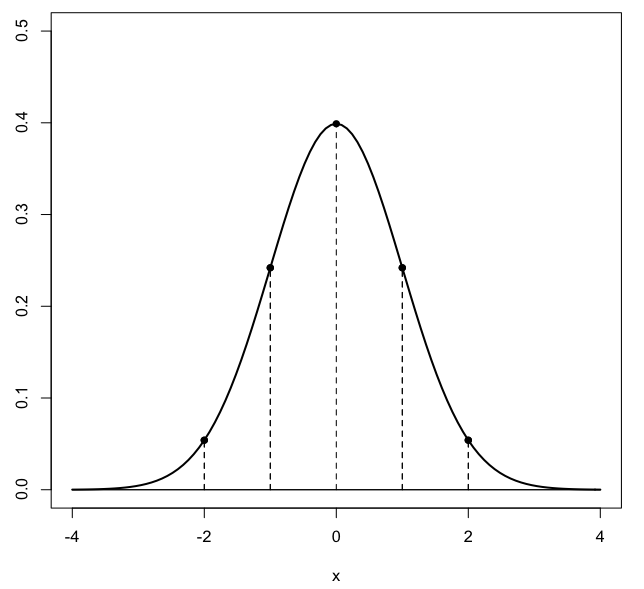
\includegraphics [scale=0.4] {gauss3.png} \end{center}

%break
\title{L'Hospital's Rule}
\date{}

\begin{document}
\maketitle
\Large

\label{sec:Hospital}

\subsection*{origin}
The rule discussed below is attributed to l'Hospital, which is also often written l'H\^{o}pital.  The latter spelling is modern French usage, while the one we use (because it is easier to typeset in titles) is English usage.  It also happens to be the way l'Hospital spelled his name himself, back in the day.

In any event, this rule was actually discovered by Johann Bernoulli.  According to Stewart, these two mathematicians had entered into a business arrangement whereby the Marquis de l'Hospital bought the rights to Bernoulli's mathematical discoveries.

\url{http://www.stewartcalculus.com/data/ESSENTIAL%20CALCULUS%20Early%20Transcendentals/upfiles/projects/ecet_wp_0307_stu.pdf}

According to wikipedia,

\begin{quote}
In the 17th and 18th centuries, the name was commonly spelled "l'Hospital", and he himself spelled his name that way. However, French spellings have been altered: the silent 's' has been removed and replaced with the circumflex over the preceding vowel (l'H\^{o}pital). The former spelling is still used in English where there is no circumflex.\end{quote}

\subsection*{limit of a quotient}

We are trying to determine the limit of the quotient of two functions
\[ \lim_{x \rightarrow c} \ \frac{f(x)}{g(x)} \]

and suppose that we run into trouble because both functions have problems at $c$.  If
\[ \lim_{x \rightarrow c} f(x) = \lim_{x \rightarrow c} g(x) = 0 \]
or 
\[ \lim_{x \rightarrow c} f(x) = \lim_{x \rightarrow c} g(x) = \infty \]
or
\[ \lim_{x \rightarrow c} f(x) = \lim_{x \rightarrow c} g(x) = -\infty \]

and if 
\[ \lim_{x \rightarrow c} \ \frac{f'(x)}{g'(x)} \]
exists

Then
\[ \lim_{x \rightarrow c} \ \frac{f(x)}{g(x)} = \lim_{x \rightarrow c} \ \frac{f'(x)}{g'(x)} \]

Here's a simple example.  What is
\[ \lim_{x \rightarrow 0} \ \frac{\sin x}{x} \]

We \emph{know} this.  it is equal to $1$.  But $\sin 0 = 0$ so take derivatives
\[ \lim_{x \rightarrow 0} \ \frac{f'(x)}{g'(x)} = \lim_{x \rightarrow 0} \frac{\cos x}{1} = 1  \]

If the limit is still of the form $0/0$ just repeat the process.

\subsection*{basic proof}
If 

$\bullet$  $f$ and $g$ are well-behaved (continuously differentiable)

$\bullet$  The first differentiation yields a finite limit as $x \rightarrow c$ and

$\bullet$  The form of the quotient is $0/0$, with $f(c) = g(c) = 0$

then

\[ \lim_{x \rightarrow c} \ \frac{f(x)}{g(x)} \]
\[ = \lim_{x \rightarrow c} \ \frac{f(x) - f(c)}{g(x) - g(c)}  \]
\[ = \lim_{x \rightarrow c} \ \frac{\ [ \ f(x) - f(c) \ ] /(x-c)}{\ [ \ g(x) - g(c) \ ] / (x-c)}  \]
\[ = \frac{\lim_{x \rightarrow c} \ [ \ f(x) - f(c) \ ] /(x-c)}{\lim_{x \rightarrow c} \ [ \ g(x) - g(c) \ ] / (x-c)}  \]
\[ = \frac{f'(x)}{g'(x)} \]

\subsection*{application to the exponential}

We will develop a proof that
\[ e = \lim_{n \rightarrow \infty} \ (1 + \frac{1}{n})^n \]
using l'Hospital's Rule.

This interesting approach is from the book \emph{Mooculus}.  Remember that $n$ is a variable in this section.

The first thing is to rewrite this as an exponential, first for the term in parentheses:
\[ 1 + \frac{1}{n} = e^{\ln(1 + 1/n)} \]
and then for the whole thing
\[ (1 + \frac{1}{n})^n =  (e^{\ln(1 + 1/n)})^n \]
\[ = \ e^{n \ln(1 + 1/n)} \]
To evaluate the limit, we need to evaluate the limit of the exponent
\[ \lim_{n \rightarrow \infty} n   \ln (1 + \frac{1}{n})  \]

At first, it doesn't look like we can use the rule (there is no quotient), but there is a standard trick for these situations.  Just rearrange to divide by the inverse
\[ = \lim_{n \rightarrow \infty} \frac{ \ln (1 + \frac{1}{n})}{\frac{1}{n}}  \]
Both the top and the bottom limits are easily evaluated to be equal to $0$, so we can apply the rule.

We need to evaluate
\[ = \lim_{n \rightarrow \infty} \frac{f'(n)}{g'(n)} \]
The derivative of the numerator is (by the chain rule)
\[ f'(n) = \frac{-n^{-2}}{1 + 1/n} \]
while the denominator is just
\[ g'(x) = -n^{-2} \]

The factor of $-n^{-2}$ cancels from both top and bottom, leaving us with
\[ \lim_{n \rightarrow \infty} \frac{1}{1 + 1/n} = 1  \]
That is:
\[ \lim_{n \rightarrow \infty} n \ \ln (1 + \frac{1}{n}) = 1 \]

Going back to the original problem then
\[ \lim_{n \rightarrow \infty} \ (1 + \frac{1}{n})^n = \lim_{n \rightarrow \infty} \  e^{n \ln(1 + 1/n)} \]
\[ = e^1 = e \]

\subsection*{exponential function}

A parallel argument can be used to prove that
\[ e^x = \lim_{n \rightarrow \infty} \ (1 + \frac{1}{n})^{nx} = \lim_{n \to \infty} (1 + \frac{x}{n})^{n} \]

with the assistance again of l'Hospital's Rule.  
 
 What we need to show is that we can bring $x$ inside the parentheses
\[ e^x =  \lim_{n \to \infty} (1 + \frac{x}{n})^{n} \]
Taking logarithms, this is the same as saying that
\[ x =  \lim_{n \to \infty} n \cdot \ln (1 + \frac{x}{n} ) \]
As before, we form the quotient
\[ \frac{\log (1 + x/n)}{1/n} \]

Use the chain rule to obtain the derivative of the numerator --- remember that $n$ is the variable:
\[ \frac{1}{1 + x/n} \ (- \frac{x}{n^2}) \]
The derivative of the denominator is $-1/n^2$ so we can cancel
\[ \frac{f'(x)}{g'(x)} = \frac{1}{1 + x/n} \ (x) \]
We take the limit
\[ \lim_{n \to \infty} \frac{1}{1 + x/n} \ (x)  = x \]

\end{document}